\newcommand{\NUMBER}{12}
\newcommand{\EXERCISES}{5}
\newcommand{\DEADLINE}{08.02.2021}
\newcommand{\COURSE}{Graphical Data}
\newcommand{\STUDENTA}{Philipp von Bachmann, \\Mat.-Nr.: 4116220}
\newcommand{\STUDENTB}{David Ott, \\Mat.-Nr.: 4185646}
\documentclass[a4paper]{scrartcl}
\usepackage[utf8]{inputenc}
\usepackage[english]{babel}
\usepackage{amsmath, enumerate, amssymb, multirow, fancyhdr, color, graphicx, lastpage, listings, tikz, pdflscape, subfigure, float, polynom, hyperref, tabularx, forloop, geometry, listings, fancybox, tikz, forest, tabstackengine, cancel, hyperref}
\input kvmacros
\geometry{a4paper,left=3cm, right=3cm, top=3cm, bottom=3cm}
\pagestyle {fancy}
\fancyhead[C]{\COURSE}
\fancyhead[R]{\today}
\fancyfoot[L]{}
\fancyfoot[C]{}
\fancyfoot[R]{Page \thepage /\pageref*{LastPage}}
\def\header#1#2{
  \begin{center}
    {\Large Assignment #1}\\
    %{(Due by: #2)}
  \end{center}
}

\newcounter{punktelistectr}
\newcounter{punkte}
\newcommand{\punkteliste}[2]{%
  \setcounter{punkte}{#2}%
  \addtocounter{punkte}{-#1}%
  \stepcounter{punkte}%<-- also punkte = m-n+1 = Anzahl Spalten[1]
  \begin{center}%
  \begin{tabularx}{\linewidth}[]{@{}*{\thepunkte}{>{\centering\arraybackslash} X|}@{}>{\centering\arraybackslash}X}
      \forloop{punktelistectr}{#1}{\value{punktelistectr} < #2 } %
      {%
        \thepunktelistectr &
      }
      #2 &  $\Sigma$ \\
      \hline
      \forloop{punktelistectr}{#1}{\value{punktelistectr} < #2 } %
      {%
        &
      } &\\
      \forloop{punktelistectr}{#1}{\value{punktelistectr} < #2 } %
      {%
        &
      } &\\
    \end{tabularx}
  \end{center}
}
\begin{document}

\begin{tabularx}{\linewidth}{m{0.3 \linewidth}X}
  \begin{minipage}{\linewidth}
    \STUDENTA\\
    \STUDENTB
  \end{minipage} & \begin{minipage}{\linewidth}
    \punkteliste{1}{\EXERCISES}
  \end{minipage}\\
\end{tabularx}
\header{Nr. \NUMBER}{\DEADLINE}

\section{De Casteljau}
  \begin{itemize}
    \item $u_0 = 0.5$\\
      \begin{align*}
          b_0^3(0.5)
          & =0.5 \cdot b_1^2(t) + 0.5 \cdot b_0^2\\
          & =0.5 \cdot (0.5 \cdot b_1^1(t) + 0.5 \cdot b_2^1) + 0.5 \cdot (0.5 \cdot b_0^1(t) + 0.5 \cdot b_1^1)\\
          & =0.5 \cdot (0.5 \cdot (0.5 \cdot b_1^0(t) + 0.5 \cdot b_0^0) + 0.5 \cdot (0.5 \cdot b_2^0(t) + 0.5 \cdot b_1^0))\\
          & + 0.5 \cdot (0.5 \cdot (0.5 \cdot b_2^0(t) + 0.5 \cdot b_1^0) + 0.5 \cdot (0.5 \cdot b_3^0(t) + 0.5 \cdot b_2^0))\\
          & =0.5 \cdot (0.5 \cdot (0.5 \cdot \begin{pmatrix}1\\ 3 \end{pmatrix}  + 0.5 \cdot \begin{pmatrix}0\\ 0 \end{pmatrix}) + 0.5 \cdot (0.5 \cdot \begin{pmatrix}3\\ 2 \end{pmatrix} + 0.5 \cdot \begin{pmatrix}1\\ 3 \end{pmatrix})) \\
          & + 0.5 \cdot (0.5 \cdot (0.5 \cdot \begin{pmatrix}3\\ 2 \end{pmatrix} + 0.5 \cdot \begin{pmatrix}1\\ 3 \end{pmatrix}) + 0.5 \cdot (0.5 \cdot \begin{pmatrix}4\\ 0 \end{pmatrix} + 0.5 \cdot \begin{pmatrix}3\\ 2 \end{pmatrix}))\\
          & =0.5 \cdot (0.5 \cdot \begin{pmatrix}0.5\\ 1.5 \end{pmatrix} + 0.5 \cdot \begin{pmatrix}2\\ 2.5 \end{pmatrix}) + 0.5 \cdot (0.5 \cdot \begin{pmatrix}2\\ 2.5 \end{pmatrix} + 0.5 \cdot \begin{pmatrix}3.5\\ 1 \end{pmatrix})\\
          & =0.5 \cdot \begin{pmatrix}1.25\\ 2 \end{pmatrix} + 0.5 \cdot \begin{pmatrix}2.25\\ 1.75 \end{pmatrix}\\
          &= \begin{pmatrix}1.75\\ 1.875 \end{pmatrix}
      \end{align*}
    \item $u_1=0.75$\\
      \begin{align*}
        b_0^1&=0.75 \begin{pmatrix}1\\ 3 \end{pmatrix} + 0.25  \begin{pmatrix}0\\ 0 \end{pmatrix} =  \begin{pmatrix}0.75\\ 2.25 \end{pmatrix}\\
        b_1^1&=0.75 \begin{pmatrix}3\\ 2 \end{pmatrix} + 0.25  \begin{pmatrix}1\\ 3 \end{pmatrix} =  \begin{pmatrix}2.5\\ 2.25 \end{pmatrix}\\
        b_2^1&=0.75 \begin{pmatrix}4\\ 0 \end{pmatrix} + 0.25  \begin{pmatrix}3\\ 2 \end{pmatrix} =  \begin{pmatrix}3.75\\ 0.5 \end{pmatrix}\\
        b_0^2&=0.75 \begin{pmatrix}2.5\\ 2.25 \end{pmatrix} + 0.25  \begin{pmatrix}0.75\\ 2.25 \end{pmatrix} =  \begin{pmatrix}2.05\\ 2.25 \end{pmatrix}\\
        b_1^2&=0.75 \begin{pmatrix}3.75\\ 0.5 \end{pmatrix} + 0.25  \begin{pmatrix}2.5\\ 2.25 \end{pmatrix} =  \begin{pmatrix}3.4375\\  0.9375 \end{pmatrix}\\
        b_0^3&=0.75 \begin{pmatrix}3.4375\\  0.9375 \end{pmatrix} + 0.25  \begin{pmatrix}2.05\\ 2.25 \end{pmatrix} =  \begin{pmatrix}3.090625\\ 1.265625 \end{pmatrix}\\
      \end{align*}
  \end{itemize}

  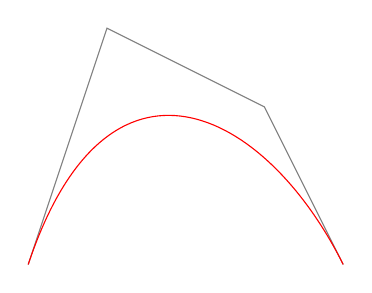
\begin{tikzpicture}
    \draw[gray] (0,0) -- (1,3) -- (3,2) -- (4,0);
    \draw[red] (0,0) .. controls (1,3) and (3,2) .. (4,0);
  \end{tikzpicture}


\section{Derivative of a Bezier Curve}
  \subsection{a)}
    \begin{align*}
      \frac{\partial P(t) }{\partial t}
      &= \frac{\partial \sum_{i=0}^n B_i^n(t) b_i}{\partial t}\\
      &= \sum_{i=0}^n  \frac{\partial B_i^n(t) b_i}{\partial t}\\
      &= \sum_{i=0}^n  b_i \frac{\partial B_i^n(t)}{\partial t}\\ % TODO: add middle part of proof
      &= n \sum_{i=0}^n B_i^{n-1}(t) (b_{i+1}-b_i)\\
    \end{align*}

  \subsection*{b)}
    Points are given as: $q_0 = 4(b_1 - b_0) = (4, 12), q_1 = (8,-2), q_2 = (4,-8)$.
    \begin{tikzpicture}[scale=0.50]
      \draw[gray] (4,12) -- (8,-2) -- (4,-8);
      \draw[red] (4,12) .. controls (8,-2) .. (4,-8);
    \end{tikzpicture}

  \subsection*{c)}
    $C^\infty$ 

\section{Hermite curves}
  \subsection*{a)}
    The points $b_0, b_3$ a simply given by $P_0, P_1$. In the lecture, we saw
    that we can convert from Bezier to Hermite via: $P'_0=3(b_1-b_0)$.
    Therefore, to get $b_1$, we can solve for it:
    \begin{align*}
      P'_0=3(b_1-b_0)\\
      P'_0/3=b_1-b_0\\
      P'_0/3 + b_0 =b_1\\
      P'_0/3 + P_0 =b_1\\
    \end{align*}
    Similar works for $b_2$.
    Therefore: 
      \begin{align*}
        G_B
        &= \begin{pmatrix}
          b_0\\b_1\\b_2\\b_3
        \end{pmatrix}\\
        &= \begin{pmatrix}
          1 & 0 & 0 & 0\\
          1 & 0 & 1/3 & 0\\
          0 & 1 & 0 & 0\\
          0 & 1 & 0 & 1/3\\
        \end{pmatrix}
        \cdot \begin{pmatrix}
          P_0\\P_1\\P'_0\\P'_1
        \end{pmatrix}
      \end{align*}

  \subsection*{b)}
    \begin{align*}
      G_H
      &= \begin{pmatrix}
        1 & 0 & 0 & 0\\
        0 & 0 & 0 & 1\\
        -3 & -3 & 0 & 0\\
        0 & 0 & -3 & -3\\
      \end{pmatrix}
      \cdot \begin{pmatrix}
        b_0\\b_1\\b_2\\b_3
      \end{pmatrix}\\
      &= \begin{pmatrix}
        1 & 0 & 0 & 0\\
        0 & 0 & 0 & 1\\
        -3 & 3 & 0 & 0\\
        0 & 0 & -3 & 3\\
      \end{pmatrix}
      \cdot \begin{pmatrix}
        0 & 0 \\ 1 & 3 \\ 3 & 2\\ 4 & 0
      \end{pmatrix}\\
      &=\begin{pmatrix}
        0 & 0 \\ 1 & 3 \\ 3 & 9 \\ 3 & -6
      \end{pmatrix}\\
    \end{align*}

\section{Splines}
  It is not possible to draw a circle with a uniform B-Spline, but it is
  possible to draw a very good apprximation of a circle, which is almost
  indistinguishable.

  This is the case, because B-Splines are defined as piecewise polynomial
  functions, which can not exactly represent the arc of a circle, which would
  require the capability to represent a square root. 


\section{Random questions}
  \subsection*{a)}
    As high frequencies represent the sharp edges in an image, applying a high
    pass filter will sharpen the edges.

  \subsection*{b)}
    The Nyquist frequency is the highest frequency that can be represented. It
    is the half of the sampling frequency. As soon as frequencies higher than
    Nyquist are present, an aliasing effect occurs.
    





\end{document}



